\section{Overview}
\label{sec:overview}
% Our general view of a distributed cps program 
% koord 3 plane arch 
     An agent in the distributed system consists of -
a $\lgname$ {\em program}, 
-a {\em controller}, and 
- a physical plant.

\begin{figure}[h!]
\centering
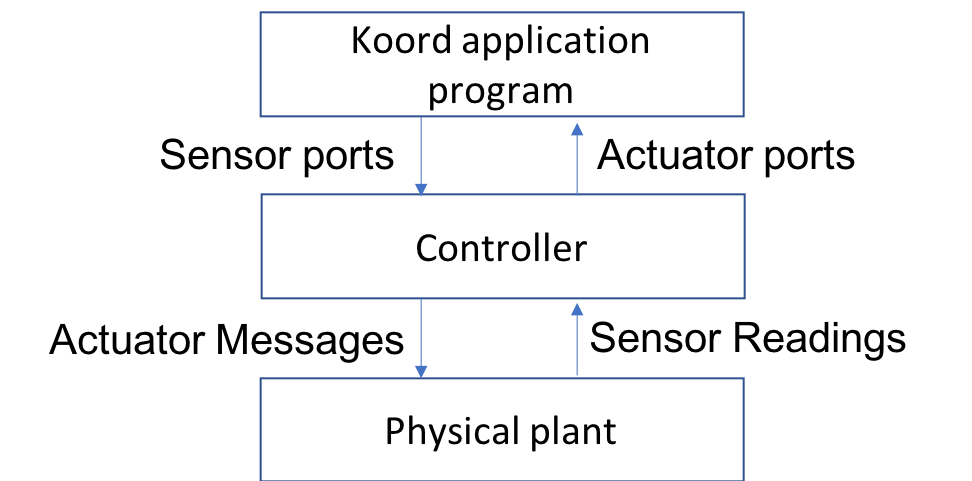
\includegraphics[width=0.48\textwidth]{figs/krdarch.png}
\caption{\small CyPhyHouse framework. Major tools shown in blue.}
\label{fig:arch}
\end{figure}
The program and the controller interact with each other through {\em sensor} and {\em actuator} ports (\reffig{arch}).  The program reads the sensor ports, reads and writes to program variables, and writes to actuator ports---represented in $\lgname$ as \emph{events} which may occur if their preconditions hold true. The controller drives the underlying physical plant. The \emph{environment} of a  $\lgname$ program is the combination of the controller and the plant. The set of agents in the system may interact with each other using {\em shared variables\/}. Each agent in the system runs an instance of the \emph{same} $\lgname$ program. 
% exmaple code snippet
\begin{figure}[ht!]
    \noindent
    \begin{mdframed}

    \begin{center}
        \scriptsize
        \two{0.4}{0.6}
        {\lstinputlisting[language=xyzNums,firstline=1,lastline=23,frame=none]{code/tasks_new.tex}}
        {\lstinputlisting[language=xyzNums,firstline=24,frame=none,firstnumber=24]{code/tasks_new.tex}}
    \end{center}
    \end{mdframed}

    \caption{$\lgname$ program for robot $i$ to do required tasks at provided locations.}
    \label{fig:taskapp}
\end{figure}
    
{\bf Task Coordination Application} \reffig{taskapp} shows a distributed task allocation application written in $\lgname$. Distributed task allocation is challenging as it involves mutual exclusion as well as construction of de-conflicted  paths. Tasks are abstractions for real location-based objectives like package delivery, surveillance, or fire-fighting.  Koord enables implementation of simple task allocation strategies using shared variables.

In $\mathit{Task}$ app, the agents maintain a shared list of tasks ({\em taskList}) to complete, and each agent is uniquely assigned a task from this list in the event {\em Assign}. Once an agent reaches the task location (event {\em Reached}), it does whatever the task entails (event {\em Complete}), and continues this process. We use the modular nature of $\lgname$ to implement dynamic path planning,  mutual exclusion through shared variables, and  collision avoidance.
% language features - what main "issue" each feature addresses . 
% organization of the rest of the paper. 


